\chapter{点云重建实验与分析}
本章介绍点云重建实验的细节、实验结果以及同其他方法的对比。实验在仿真数据和真实数据上均进行了验证。训练和定量的分析用到了两个人体数据集,一个是将动作捕捉序列拟合到SMPL参数化模型\citep{loper2015smpl}上生成的人体模型数据,另一个是真实人体通过多视角重建技术扫描得到的Twindom数据集。本方法与传统方法\citep{kazhdan2006, kazhdan2013}以及最新的基于深度学习的点云重建方法\citep{Chibane_2020_CVPR}进行了比较。实验证明新方法的鲁棒性在视觉效果和定量指标方面都优于这些方法。为了测试泛化性能,还进行了两个数据集之间的交叉测试实验。
真实数据由Kinect Azure搭建的采集系统获取,实验结果说明与传统方法相比,本方法具有良好的鲁棒性和泛化性能。

\section{实验环境和设置}
主机为64位x86架构机器,使用单张NVIDIA TITAN X显卡。网络使用PyTorch框架实现,可导渲染模块使用Pytorch3D实现。SMPL数据集的人体模型具有不同的姿态和形状,但是身体表面光滑,没有如衣服褶皱等高频信息,在所有的动作序列中采样导出了800个人体模型,所有模型具有同样的拓扑。Twindom数据集的人体模型姿态多为静态站立,由于采用多视角重建的方法恢复几何,衣服等几何细节保留逼真。从中随机挑出1200个模型,包括多种不同的复杂衣服、发型和形态。单个原始Twindom模型的顶点数量多达50万的量级,需要首先进行简化,将其顶点数量降到10万以下,同时严格保持模型质量几乎不受损。对于所有数据集,每个模型上采样点云的点数为20000,空间点集的采样数为5000。训练SMPL数据集和Twindom数据集的时间均在12小时左右,这包括了第一阶段的单视角训练和第二阶段的多视角调优。

\section{量化结果的比较}
在SMPL数据集和Twindom数据集,再加上各自模拟噪声产生的共四个数据集上,对比测试了单视角训练和多视角调优的效果,同时还对比了泊松重建和IFnet的表现。定量指标采用点云重建结果到真实模型的距离来衡量。给定点云$P$重建得到的几何$M_P$,对其上各顶点$v$,计算$v$到真实模型表面$M$的最近距离并求其均值,如公式(\ref{eq:pc_measure})所示。其中$|M_p|$表示重建出的几何包含的顶点数目。
\begin{equation} \label{eq:pc_measure}
    \adddotsbeforeeqnnum%
    D = \frac{1}{|M_p|}\sum_{v \in M_p} \|v - \mathrm{argmin}_{u\in M}\|v - u\|_2\|_2^2
\end{equation}

表\ref{tab:pc_measure}展示了依照此度量计算出的各个方法在数据集上的表现。可以看出,在没有噪声的情况下,泊松重建要明显优于深度学习的方法,这是因为点云的均匀采样如实反映出了模型的几何信息。然而在加入噪声后,泊松重建的结果会严重受到噪声影响,相反数据驱动的方法能够从训练数据中学习到去噪与补全缺损的方法,具有很好的鲁棒性。同时本方法采取的多视角投影提取几何信息的方式比直接从点云周围提取信息的IFnet表现更好。
\begin{table}[!htbp]
\bicaption[四个数据集上重建误差对比]{四个数据集上重建误差对比。Ours-s表示单视角训练结果,Ours-m表示多视角调优后的结果。真实模型尺度被缩放到单位1之内,距离值越小,重建效果越好。结果数据$\times 10^3$。}[Reconstruction loss of all methods on four datasets]{Reconstruction loss of all methods on four datasets. Ours-s is trained with single view supervision and Ours-m is refined with multi-view setting. The ground-truth models are scaled to uniform sphere. Smaller value implies better performance. Results $\times 10^3$.}
\label{tab:pc_measure}
\centering
\footnotesize% fontsize
\setlength{\tabcolsep}{4pt}% column separation
\renewcommand{\arraystretch}{0.9}%row space 
\begin{tabular}{c c c c c}
\hline\noalign{\smallskip}
Method  & Poisson & IFnet & Ours-s & Ours-m \\
\noalign{\smallskip}
\hline
\noalign{\smallskip}
SMPL   & \textbf{0.43} & 2.56 & 3.49 & 0.81 \\
SMPL+Noise & 1.34 & 1.73 & \textbf{1.17} & \textbf{0.92}\\
Twindom & \textbf{1.02} & 2.84 & 2.89 & 1.97 \\
Twindom+Noise & 3.43 & 2.74 &\textbf{1.84} & \textbf{1.36}\\
\hline
\end{tabular}
\end{table}

对比本方法在单视角训练和多视角调优的结果,可以发现经过多视角调优之后在各个数据集上的重建效果都会更好。SMPL数据集和Twindom数据集在单视角下,训练数据中加入噪声之后重建效果在数据上反而比不加噪声的时候表现更优,这可能是由于在添加噪声的情况下去噪和补洞操作都倾向于向均值回归,使得重建出的模型到真实模型的距离变小。

\section{可视化结果的比较}
图\ref{fig:pc_visual}展示了不同方法在两个数据集上的重建结果示例。SMPL
数据集的人体比较光滑,没有衣服纹理,而Twindom数据集的衣服纹理和头发细节更丰富。泊松重建对于细小结构例如手指等在采样密度不够的时候无法正确计算法向,因而无法准确重建相应结构。本方法的单视角重建结果能够恢复出大概的人体形状,即便无法恢复细节,也能大概补全出正确的轮廓,而经过多视角调优后能够获得更加精细的重建结果,对于比较精细的几何结构也取得了比传统方法更好的效果。

\begin{figure}
    \centering
    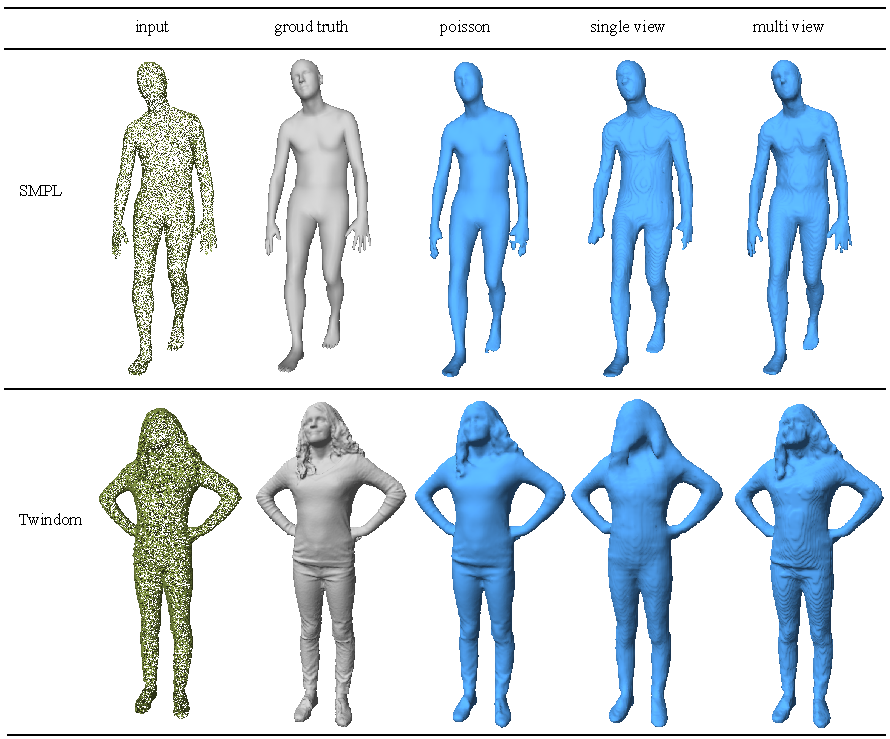
\includegraphics[width=\textwidth]{visual_result_pc.pdf}
    \bicaption[各方法在两个数据集上的点云重建结果对比]{各方法在两个数据集上的点云重建结果对比。单视角表示仅经过单视角训练,多视角 表示经过多视角调优后的结果。}[Results of different methods on SMPL and Twindom dataset]{Results of different methods on SMPL and Twindom dataset. “Single view” indicates the network is trained with single-view supervision only and "multi view" indicates the network is refined with multi-view setting.}
    \label{fig:pc_visual}
\end{figure}


\begin{figure}
    \centering
    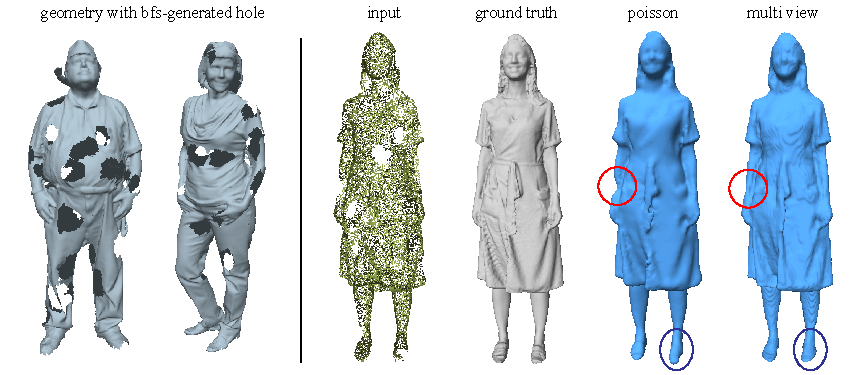
\includegraphics[width=\textwidth]{noise_pc.pdf}
    \bicaption[叠加模拟噪声后各方法的重建效果对比]{叠加模拟噪声后各方法的重建效果对比。圆圈区域显示了传统重建方法无法恢复而新方法能够正确推测并补全缺损的情况。}[Results of different methods when adding noise to geometry]{Results of different methods when adding noise to geometry. The circles indicates cases traditional methods failed to reconstruct while our method generalizes well.}
    \label{fig:pc_noise}
\end{figure}

\begin{figure}
    \centering
    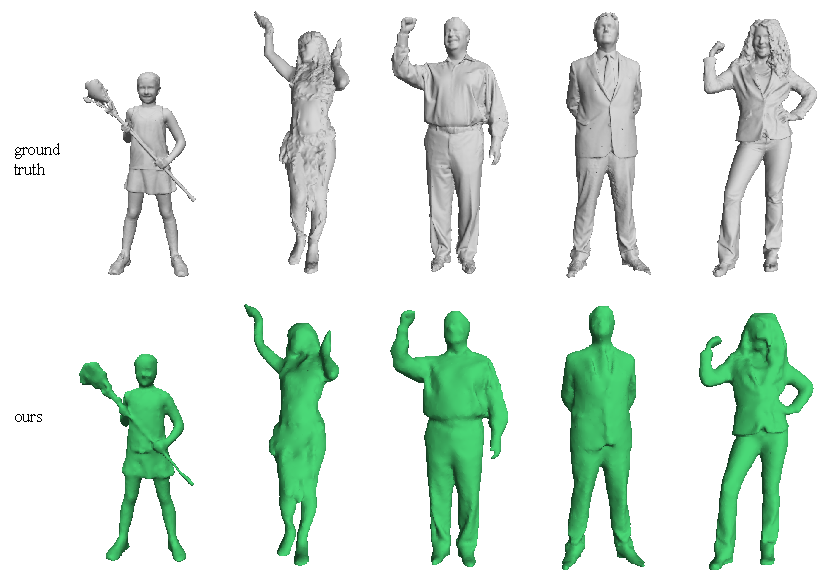
\includegraphics[width=\textwidth]{more_twindom_results.pdf}
    \bicaption[更多Twindom上的结果]{更多Twindom数据集上的结果。第一行为真实模型,第二行为本方法在Twindom数据集上的结果}[More results of Twindom dataset]{More results of Twindom dataset. The first line shows the ground truth data, the second line shows our results.}
    \label{fig:pc_more_twindom}
\end{figure}

图\ref{fig:pc_noise}展示了叠加模拟噪声的可视化结果。左边展示了Twindom训练集上通过BFS生成的空洞,右边对比了在测试数据上不同方法的结果。泊松重建由于缺乏数据先验,在较大面积缺损的情况下,从点云重建出的几何出现明显的瑕疵,而新方法在训练过程中对噪声和缺损有了先验,在测试数据上能保持较好的鲁棒性和泛化性,注意测试用的数据在训练过程中网络并未见过。

\section{数据集的交叉测试对比}
\begin{figure}[!htbp]
    \centering
    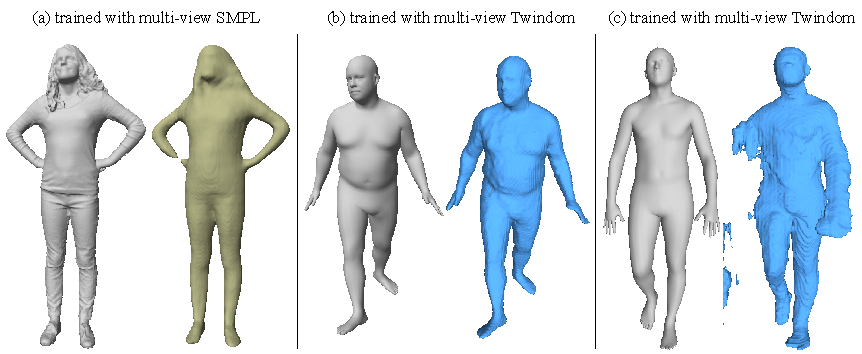
\includegraphics[width=\textwidth]{dataset_cross_pc.pdf}
    \bicaption[SMPL和Twindom交换测试集的结果对比]{SMPL和Twindom交换测试集的结果对比。(a)中模型在SMPL上多视角训练,在Twindom上多视角测试;(b)中模型在Twindom上多视角训练,在SMPL上多视角测试;(c)中模型在Twindom上多视角训练,在SMPL上单视角测试。}[Results of exchanging testing data on SMPL and Twindom dataset]{Results of exchanging testing data on SMPL and Twindom dataset. (a) The model is trained on SMPL (multi-view) and test on Twindom (multi-view); (b) The model is trained on Twindom (multi-view) and test on SMPL (multi-view); (c) The model is trained on Twindom (multi-view) and test on SMPL (single view).}
    \label{fig:pc_data_cross}
\end{figure}
为了比较隐函数在不同数据集上的表现差异以及验证网络的泛化性能,在SMPL和Twindom数据上进行了交叉测试,即用一个数据集的测试数据测试在另一个数据集上训练过的模型。图\ref{fig:pc_data_cross}展示了测试结果,当模型在SMPL数据集上训练之后,Twindom上的重建结果会过于平滑,衣服、头发和面部的几何细节明显丢失。当模型先在Twindom数据集上训练后,SMPL数据集的重建结果增加了部分细节,但是同时也引入了一些多余的细节,原本光滑的皮肤位置多出了很多褶皱。值得注意的是Twindom上经过多视角调优的网络,在SMPL上进行单视角测试时,出现了过多的噪声,甚至无法恢复出基本的形状信息,这说明隐函数对几何细节的学习和对噪声的容忍是存在权衡的,当数据倾向于表达更多细节时,隐函数模块更容易过拟合以保证丰富的细节。



\section{真实数据的测试结果}
采集系统由六个Kinect Azure设备构成,大致分布在一个直径为3米的圆周上,环绕着中间的拍摄物体,能够同步采集RGBD数据流。相机的位置参数通过预标定过程获得。采集得到的深度图充斥着噪声和由于遮挡变化导致的空洞,如图\ref{fig:pc_kinect_depth}所示。
\begin{figure}[!htbp]
    \centering
    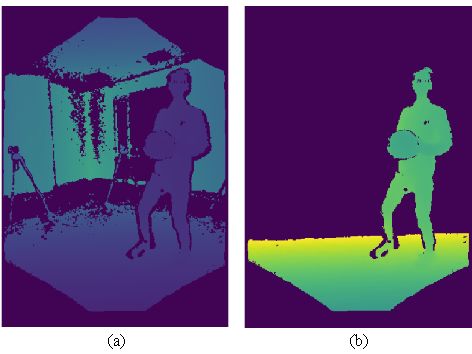
\includegraphics[width=0.6\textwidth]{kinect_depth.pdf}
    \bicaption[Kinect深度图的原始输入及预处理]{Kinect深度图的原始输入及预处理。(a)Kinect Azure原始深度图; (b)预处理结果。}[Raw Kiect depth map and results after pre-processing]{Raw Kiect depth map and results after pre-processing. (a) raw output of Kinect Azure; (b) result after pre-processing.}
    \label{fig:pc_kinect_depth}
\end{figure}
同时各个相机的标定过程产生的误差使得深度图无法完全对齐,图\ref{fig:pc_kinect_pointcloud}展示了从六个相机直接融合得到的点云,放大部分强调了三个导致点云质量差的主要原因:遮挡造成的空洞,标定误差造成的不对齐和离群噪声点。鉴于本方法对输入点云首先要投影到各个视角得到深度图,这使得Kinect采集到的深度图刚好可以直接作为编码器的输入。

图\ref{fig:pc_kinect_result}展示了重建结果。在获取的单帧点云质量较差的情况下,泊松重建无法处理噪声,所有的标定误差和噪声毛刺在重建结果中都依然存在,放大的局部细节中头部点云的大片空洞几何显得杂乱。而本方法使用了Twindom上预训练的模型,在噪声比较严重的情况下,保持了基本的形状和几何的平滑度,对于头部相机没有采到的区域,能够合理补全出头部形状,虽然模型本身有些过度平滑,但考虑到噪声和细节的权衡,得到的结果比传统方法明显更能让人接受。

\section{本章小结}

本章介绍了多视角投影结合隐函数的点云重建方法的实验结果。通过在SMPL数据集和Twindom 数据集上的测试,验证了方法的有效性。通过与其他方法的定量和观感上的对比,说明了本方法重建质量的优越性,尤其是对噪声和空洞等瑕疵的鲁棒性。通过在真实kinect数据上的测试,说明了新方法的泛化性和鲁棒性。

\begin{figure}[!htbp]
    \centering
    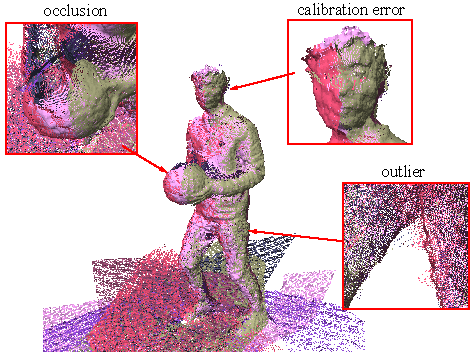
\includegraphics[width=0.7\textwidth]{kinect_pointcloud.pdf}
    \bicaption[六相机融合点云]{六相机融合点云。不同颜色代表来自不同相机的点云。放大部分展示了三个影响点云质量的因素。}[Raw pointclouds directly fused from six cameras]{Raw pointclouds directly fused from six cameras. Different color indicates the part of points are from different cameras. The three closeups shows the main cause of the artifacts.}
    \label{fig:pc_kinect_pointcloud}
\end{figure}

\begin{figure}[!htbp]
    \centering
    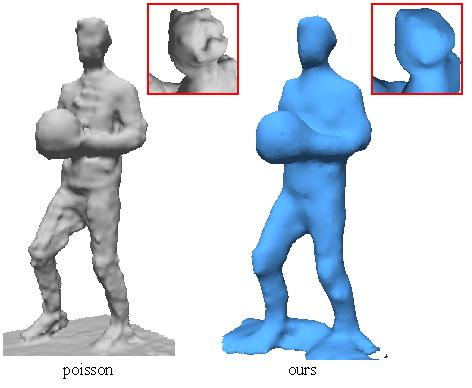
\includegraphics[width=0.65\textwidth]{kinect_result.pdf}
    \bicaption[Kinect数据的重建结果对比]{Kinect数据的重建结果对比。左边是泊松重建的结果,右边是本方法在Twindom上训练后对kinect数据的重建结果。}[Reconstruction results of Kinect data]{Reconstruction results of Kinect data. The left is result of poisson reconstruction, and the right is the results of our method trained with Twindom dataset.}
    \label{fig:pc_kinect_result}
\end{figure}